\documentclass{article}
\usepackage[utf8]{inputenc}
\usepackage{graphicx}
\graphicspath{ {images/} }
\usepackage{fullpage}
\usepackage{float}
\usepackage{subcaption}
\usepackage{listings}
\usepackage{paralist}
\usepackage{xcolor}
\lstnewenvironment{longlisting}[1][ML] 
  {\noindent\minipage{\textwidth}
    \lstset{
      basicstyle=\ttfamily\footnotesize,
      columns=fullflexible,
      language= #1,
      frame=single,
      breaklines=true,
      postbreak=\mbox{\textcolor{gray}{$\hookrightarrow$}\space},
      backgroundcolor=\color{white},
      commentstyle=\color{magenta},
      keywordstyle=\color{blue},
      stringstyle=\color{olive}
    }
  } 
  {\endminipage}

\begin{document}
\title{Mergeable Types Library - Report}
\author{Samodya Abeysiriwardane}
\maketitle
\newpage
\tableofcontents
\newpage
\section{Abstractions and Data structures}
In our library we have implemented selected abstractions using different data structure implementations.

\begin{table}[ht]
\centering
\begin{tabular}{|l l|}
\hline
\textbf{Abstraction} & \textbf{Datastructure} \\ \hline
Vector & List \\ \hline
Set & \begin{tabular}[c]{@{}l@{}}AVL Tree\end{tabular} \\ \hline
Map & \begin{tabular}[c]{@{}l@{}}AVL Tree\\ Trie\end{tabular} \\ \hline
Heap & \begin{tabular}[c]{@{}l@{}}Leftist Heap\\ Binomial Heap\\ Pairing Heap\end{tabular} \\ \hline
\end{tabular}
\end{table}

\subsection{Framework for mergeable types} \label{mtype-framework}
To define 3-way mergeable data structures, we follow the framework illustrated in \ref{fig:merge-square}.
\begin{figure}[ht]
\centering
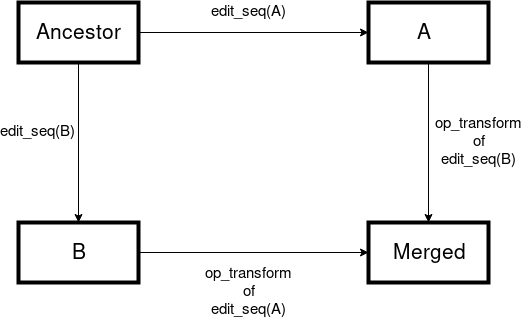
\includegraphics[width=0.7\textwidth]{merge-square.png}
\caption{\lstinline{P, Q = edit_sequence from Ancestor to A, B} and \\
\lstinline{P', Q' = operational transform of P, Q}}
\label{fig:merge-square}
\end{figure}

\newpage
We can choose to define the Edit sequence operations using the Abstraction operations, 
independent from the implementation.

\begin{table}[ht]
\centering
\begin{tabular}{|l l|}
\hline
\textbf{Abstraction} & \textbf{Edit Sequence Structures} \\ \hline
Vector & \begin{tabular}[c]{@{}l@{}}Insert (i, E)\\ Replace (i, A, E) \\ Remove(i)\end{tabular} \\ \hline
Set & \begin{tabular}[c]{@{}l@{}}Add (E)\\ Remove(E)\end{tabular} \\ \hline
Map & \begin{tabular}[c]{@{}l@{}}Add(K, E)\\ Remove(K)\\ Replace(K, A, E)\end{tabular} \\ \hline
Heap & \begin{tabular}[c]{@{}l@{}}Delete-Min (E)\\ Insert (E)\end{tabular} \\ \hline
\end{tabular}
\end{table}

\lstinline{op_transform} takes a pair of edit sequences \lstinline{s1} and \lstinline{s2}, 
that map a structure \lstinline{v} to two different structures \lstinline{v1} and \lstinline{v2}, 
and transforms \lstinline{s1} to \lstinline{s1'} such that \lstinline{s1'} has the same effect on 
\lstinline{v2} as \lstinline{s1} had on \lstinline{v}.

\subsection{Merge function}
Given ancestor, A and B versions, we can define the merge function as a composition of edit sequences 
(\lstinline{diff}) and \lstinline{op_transform}. 

\begin{longlisting}
merge3 ancestor a b:
  # p is the edit sequence from ancestor to a
  p = diff ancestor a
  # q is the edit sequence from ancestor to b
  q = diff ancestor b
  # op_transform as described above
  p', q' = op_transform p q
  # apply the transformed edit sequence of q on version a
  apply a q'
  # Note that due to commutativity of merge
  # apply a q' = apply b p'
\end{longlisting}

\newpage
\section{Vector}
\subsection{Vector signature}
\begin{longlisting}
module type Base = sig
  type atom
  type t
  val empty: t
  val length : t -> int
  val set : t -> int -> atom -> t
  val get : t -> int -> atom
  val insert : t -> int -> atom -> t
  val delete : t -> int -> t
end
\end{longlisting}

\subsection{Vector - List implementation}
Simple Vector implementation using the Lists from Ocaml stdlib. 
All Vector operations can be performed with O(n) time complexity.

\subsubsection{Edit sequence generation}
The edit sequence algorithm corresponds to the minimum edit distance between two lists, which can be computed in 
polynomial time (Wagner and Fischer 1974).

\begin{longlisting}[python]
diff v1 v2:
  # For all i and j, d[i, j] = holds the tuple of
  # min edit distance, min edit sequence of v1[:i], v2[:j]
  # Note that d has (m+1) x (n+1) values.
  let d be a 2-d array of int with dimensions [0..m, 0..n]
 
  for i in [0..m]
    # The distance of any first string to an empty snd string
    # (transforming the string of the first i characters of s into
    # the empty string requires i deletions)
    d[i, 0] = i, snd d[i-1, 0] :: Delete v1[i]
  for j in [0..n]
    d[0, j] = j, snd d[0, j-1] :: Insert v2[j]
 
  for j in [1..n]
    for i in [1..m]
      if s[i] = t[j] then  
        d[i, j] = d[i-1, j-1], snd d[i-1, j-1]
      else
        d[i, j] = minimum of
        (
          d[i-1, j] + 1, snd d[i-1, j] :: Delete v1[i]
          d[i, j-1] + 1, snd d[i, j-1] :: Insert v2[j]
          d[i-1, j-1] + 1, snd d[i-1, j-1] :: Subs v1[i], v2[j]
        )
 
  return d[m,n]
\end{longlisting}

\subsubsection{Edit sequence in action}
Please refer to \ref{vector-example} for complete usage example.

\begin{longlisting}
let module M = Mvector_list.Make(CharAtom) in

let original = ['h';'e';'l';'l';'o'] in
let v1 = ['h';'i';'l';'l';'o'] in
let v2 = ['h';'e';'l';'l';'o';'w';'o';'r';'l';'d'] in

(* Edit seq generation demonstration *)
let edit_seq_printer = U.string_of_list (M.edit_to_string CharAtom.to_string) in 
(* edit seq generation with diff *)
let p = M.op_diff original v1 in
let q = M.op_diff original v2 in
let _ = 
  Printf.printf "p = diff original v1: %s\n" (edit_seq_printer p);
  Printf.printf "q = diff original v2: %s\n" (edit_seq_printer q)

(*** Output ***)
p = diff original v1: [ Rep (1, e, i); ]
q = diff original v2: [ Ins (4, o); Ins (4, w); Ins (5, r); Ins (5, l); Ins (5, d); ]
\end{longlisting}

\subsection{Operational transform}
Given edit sequences as in \ref{mtype-framework}: 
\begin{itemize}
\item Order of the elements is retained. 
\item Non conflicting substitution at a position is a substitution operation in s1'.
\item Substitution conflict with a deletion is a no-op in s1', so that deletion wins for the final merged vector. 
\item Substitution conflict with another substitution is handled by a user defined merge of the atomic value in s1'. 
\end{itemize}
The operational transform algorithm has a complexity of O(m + n) where m, n are lengths of the edit sequences.

\begin{longlisting}
let op_transform p q =
  let cons2 (x,y) (xs,ys) = (x::xs, y::ys) in
  let rec go xs a ys b =
    match xs, a, ys, b with
    | [], _, [], _ -> ([], [])
    | xs, a, [], _ -> (shift_patch [] a xs, [])
    | [], _, ys, b -> ([], shift_patch [] b ys)
    | x::xs, a, y::ys, b ->
      (* Depending the edit operation's edit index shift the indices of p or q *)
      if index x < index y then
        let p',q' = go xs a (y::ys) (b + offset x) in
        (shift_edit a x::p',q')
      else if index x > index y then
        let p',q' = go (x::xs) (a + offset y) ys b in
        (p',shift_edit b y::q')
      (* If the indices match we recognise this as a conflict and try to resolve *)
      else begin
        match x,y with
        | _ when x = y -> go xs (a + offset y) ys (b + offset x)
        | Ins (i,nx), Ins (_, ny) ->
          (* User defined resolve function is used 
             when there is a conflict without an ancestor for an atom*)
          let n = Atom.resolve nx ny in
          cons2 (Rep (i+a,ny,n), Rep (i+b,nx,n)) (go xs (a + offset y) ys (b + offset x))
        | Rep (i, anc, nx), Rep (_, _, ny) ->
          (* User defined merge function is used 
             when there is a conflict with a known ancestor an atom *)
          let n = Atom.merge3 ~ancestor:anc nx ny in
          cons2 (Rep (i + a, ny, n), Rep (i + b, nx, n)) (go xs a ys b)
        | Ins _, _ ->
          let p',q' = go xs a (y::ys) (b + offset x) in
          (shift_edit a x::p',q')
        | _, Ins _ ->
          let p',q' = go (x::xs) (a + offset y) ys b in
          (p', shift_edit b y::q')
        | Rep (i,_,nx), Del _ ->
          let p',q' = go xs (a + offset y) ys b in
          (p', Del (i+b, nx)::q')
        | Del _, Rep (i, _, ny) ->
          let p',q' = go xs a ys (b + offset x) in
          (Del (i+a,ny)::p',q')
        | Del _, Del _ -> go xs (a + offset y) ys (b + offset x)
      end
  in
  go p 0 q 0
\end{longlisting}

\subsection{Example}\label{vector-example}
\subsubsection{Vector - List}
\begin{longlisting}
let module CharAtom = struct
  type t = char

  (* User defined merges for atom values *)
  let resolve x y = '#'
  let merge3 ~ancestor x y = '#'

  (* Used for presentation purposes *)
  let to_string c = String.make 1 c
end in

let module M = Mvector_list.Make(CharAtom) in

let original = ['h';'e';'l';'l';'o'] in
let v1 = ['h';'i';'l';'l';'o'] in
let v2 = ['h';'e';'l';'l';'o';'w';'o';'r';'l';'d'] in

(* Edit seq generation demonstration *)
let edit_seq_printer = U.string_of_list (M.edit_to_string CharAtom.to_string) in 
(* edit seq generation with diff *)
let p = M.op_diff original v1 in
let q = M.op_diff original v2 in
let _ = 
  Printf.printf "p = diff original v1: %s\n" (edit_seq_printer p);
  Printf.printf "q = diff original v2: %s\n" (edit_seq_printer q)
in
(* op_transform demonstration *)
let p', q' = M.op_transform p q in
let _ = 
  Printf.printf "p' = transformed p: %s\n" (edit_seq_printer p');
  Printf.printf "q' = transformed q: %s\n" (edit_seq_printer q')
in

let m = M.merge3 ~ancestor:original v1 v2 in

Printf.printf "merged = apply q' on v1: %s\n" (U.string_of_list CharAtom.to_string m)

(*** Output ***)
Vector - List
p = diff original v1: [ Rep (1, e, i); ]
q = diff original v2: [ Ins (4, o); Ins (4, w); Ins (5, r); Ins (5, l); Ins (5, d); ]
p' = transformed p: [ Rep (1, e, i); ]
q' = transformed q: [ Ins (4, o); Ins (4, w); Ins (5, r); Ins (5, l); Ins (5, d); ]
merged = apply q' on v1: [ h; i; l; l; o; w; o; r; l; d; ]
\end{longlisting}

\subsubsection{Vector - User defined}
\begin{longlisting}
let module M = struct
  module CharAtom = struct
    type t = char
    (* User defined merges for atom values *)
    let resolve x y = '#'
    let merge3 ~ancestor x y = '#'
    (* Used for presentation purposes *)
    let to_string c = String.make 1 c
  end
  (* User defined Vector implementation *)
  module V = struct
    type atom = char
    type t = string
    let empty = ""
    let length = String.length
    let set t i a =
      assert (0 <= i && (i + 1) <= String.length t);
    let get = String.get
    let insert t i c =
      (* truncated for clarity *)
    let delete t i =
      (* truncated for clarity *)
  end

  module Mstring = Mvector.Make(CharAtom)(V)
  include Mstring
end in

let original = "hello" in
let v1 = "hillo" in
let v2 = "helloworld" in

(* Edit seq generation demonstration *)
let edit_seq_printer = U.string_of_list (M.edit_to_string M.CharAtom.to_string) in
(* edit seq generation with diff *)
let p = M.op_diff original v1 in
let q = M.op_diff original v2 in
let _ = 
  Printf.printf "p = diff original v1: %s\n" (edit_seq_printer p);
  Printf.printf "q = diff original v2: %s\n" (edit_seq_printer q)
in
  (* op_transform demonstration *)
  let p', q' = M.op_transform p q in
  let _ = 
    Printf.printf "p' = transformed p: %s\n" (edit_seq_printer p');
    Printf.printf "q' = transformed q: %s\n" (edit_seq_printer q')
  in

let m = M.merge3 ~ancestor:original v1 v2 in

Printf.printf "merged = apply q' on v1: %s\n" m

(*** Output ***)
p = diff original v1: [ Rep (1, e, i); ]
q = diff original v2: [ Ins (4, o); Ins (4, w); Ins (5, r); Ins (5, l); Ins (5, d); ]
p' = transformed p: [ Rep (1, e, i); ]
q' = transformed q: [ Ins (4, o); Ins (4, w); Ins (5, r); Ins (5, l); Ins (5, d); ]
merged = apply q' on v1: hilloworld
\end{longlisting}

\newpage
\section{Set}
\subsection{Set signature}
This is a simplified Set signature. 

\begin{longlisting}
module type Base = sig
  type t
  type atom
  val empty: t
  val is_empty: t -> bool
  val mem: atom -> t -> bool
  val add: atom -> t -> t
  val remove: atom -> t -> t
end
\end{longlisting}

\subsection{Set - AVL tree implementation}
Ordered Set implementation from the Ocaml standard library is reused. The AVL tree has a height balancing factor of 2. 
All basic operations have O(log n) time complexity.

\subsubsection{Edit sequence generation}\label{set-avlt-diff}
This algorithm is an adaptation of (Brown and Tarjan 1977) Fast BST Merging Algorithm. 
Given two BSTs where the size is m and n and $(m < n)$ then the time complexity will be $O(mlog(n/m) + (n - m))$

An optimization we can do to gain major performance improvements in a content addressable storage 
is by doing structural comparison of the child trees before recursion. Basically if s1.hash == s2.hash, 
then the edit sequence is empty. This is an optimization that cannot be performed if another solution that used 
flattens the tree structure was used.

\begin{longlisting}[python]
diff t1 t2:
  # Base cases:
     Empty tree vs Some tree -> 
     	fold tree in-order 
     	  mark all as Add operations
     Some tree vs Empty tree ->
     	fold tree in-order 
     	  mark all as Remove operations
  # Recursive case:
     xx, r, yy = split the larger tree by root
     x,exists,y = split the smaller tree by r
     smaller = diff x x
  	 larger = diff y y
     if exists: 
     	smaller + larger
     else:
     	if t1 is larger tree then 
        	edit_op = Remove r
            smaller + [edit_op] + larger
        else 
        	edit_op = Add r
        	smaller + [edit_op] + larger
\end{longlisting}

\subsubsection{Edit sequence in action}
Refer to \ref{set-example} for complete usage example.

\begin{longlisting}
let module M =  Mset_avltree.Make(IntAtom) in

let original = M.empty |> M.add 10 |> M.add 5 |> M.add 20 in
let v1 = original |> M.add 40 |> M.add 60 |> M.remove 10 in
let v2 = original |> M.add 4 |> M.add 3 |> M.add 2 |> M.add 1 in

(* Edit seq generation demonstration *)
let edit_seq_printer = U.string_of_list (M.edit_to_string IntAtom.to_string) in
(* edit seq generation with diff *)
let p = M.op_diff original v1 in
let q = M.op_diff original v2 in
let _ = 
  Printf.printf "p = diff original v1: %s\n" (edit_seq_printer p);
  Printf.printf "q = diff original v2: %s\n" (edit_seq_printer q)

(*** Output ***)
p = diff original v1: [ Remove (10); Add (40); Add (60); ]
q = diff original v2: [ Add (1); Add (2); Add (3); Add (4); ]
\end{longlisting}

\subsection{Operational transform}
Given A ancestor set, X version and Y version set: merged set will be A + X + Y - (A - X) - (A - Y).
To achieve this merged set, given edit sequences according to \ref{mtype-framework}: 
All Set Inserts and Removes performed by s1 can be directly applied on v2, and hence be included in s1'. 
In operational transformation we can identify few cases that can be optimized to so that s1' sequence is shorter.
\begin{itemize}
\item Inserts of equal values in both sequences, is a no-op in s1'
\item. Removes of equal values in both sequences is a no-op in s1'
\item Insert and Remove of equal values is not possible because of Set's uniqueness property.
\end{itemize}

\begin{longlisting}
let op_transform p q =
  let rec transform_aux xs ys =
    match xs, ys with
    | [], [] -> [], []
    | [], _ -> [], ys
    | _, [] -> xs, []   
    | hx::rxs, hy::rys ->
      let handle kx ky on_conflict =
        (* Recognize a conflict when two atoms have equal values *)
        let c = Atom.compare kx ky in
        if c = 0 then on_conflict ()
        (* If no conflict replicate the effect of one seq on the other  *)
        else if c < 0 then 
          let a, b = transform_aux rxs ys in
          hx::a, b
        else (* c > 0 *)
          let a, b = transform_aux xs rys in
          a, hy::b in
      match hx, hy with
      | Add x, Add y
      | Remove x, Remove y ->
        let on_conflict () = transform_aux rxs rys in
        handle x y on_conflict
      | Add x, Remove y 
      | Remove x, Add y ->
        (* Impossible condition *)
        let on_conflict = fun () -> assert false in
        handle x y on_conflict
  in
  transform_aux p q
\end{longlisting}

\subsection{Example}\label{set-example}
\begin{longlisting}
let module IntAtom = struct
  type t = int
  let compare = Pervasives.compare
  (* Used for presentation purposes *)
  let to_string = string_of_int
end in

let module M =  Mset_avltree.Make(IntAtom) in

let original = M.empty |> M.add 10 |> M.add 5 |> M.add 20 in
let v1 = original |> M.add 40 |> M.add 60 |> M.remove 10 in
let v2 = original |> M.add 4 |> M.add 3 |> M.add 2 |> M.add 1 in

(* Edit seq generation demonstration *)
let edit_seq_printer = U.string_of_list (M.edit_to_string IntAtom.to_string) in
(* edit seq generation with diff *)
let p = M.op_diff original v1 in
let q = M.op_diff original v2 in
let _ = 
  Printf.printf "p = diff original v1: %s\n" (edit_seq_printer p);
  Printf.printf "q = diff original v2: %s\n" (edit_seq_printer q)
in
  (* op_transform demonstration *)
  let p', q' = M.op_transform p q in
  let _ = 
    Printf.printf "p' = transformed p: %s\n" (edit_seq_printer p');
    Printf.printf "q' = transformed q: %s\n" (edit_seq_printer q')
  in

let m = M.merge3 ~ancestor:original v1 v2 in

Printf.printf "merged = apply q' on v1: %s\n" (U.string_of_list IntAtom.to_string (M.elements m))

(*** Output ***)
p = diff original v1: [ Remove (10); Add (40); Add (60); ]
q = diff original v2: [ Add (1); Add (2); Add (3); Add (4); ]
p' = transformed p: [ Remove (10); Add (40); Add (60); ]
q' = transformed q: [ Add (1); Add (2); Add (3); Add (4); ]
merged = apply q' on v1: [ 1; 2; 3; 4; 5; 20; 40; 60; ]
\end{longlisting}

\begin{figure}[H]
  \begin{subfigure}{\linewidth}
  \begin{center}
  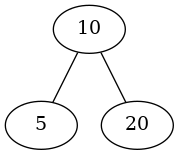
\includegraphics[height=.2\textheight,keepaspectratio]{set-avl-original.png}
  \end{center}
  \caption{Original tree}
  \end{subfigure}\par\medskip
  \begin{subfigure}{\linewidth}
  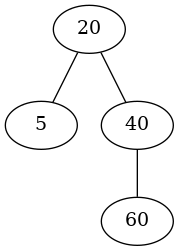
\includegraphics[width=.3\linewidth, height=.3\textheight,keepaspectratio]{set-avl-v1.png}\hfill
  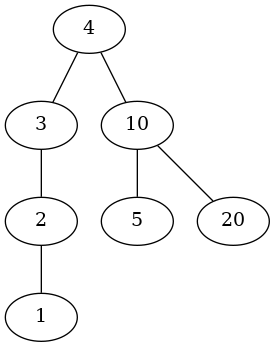
\includegraphics[width=.4\linewidth,height=.4\textheight,keepaspectratio]{set-avl-v2.png}
  \caption{v1 and v2 on left and right respectively}
  \end{subfigure}\par\medskip
  \begin{subfigure}{\linewidth}
  \begin{center}
  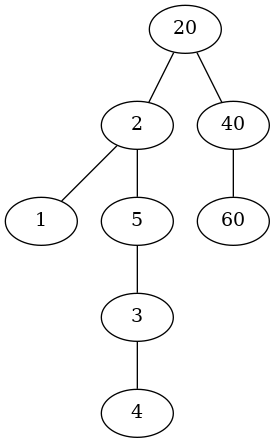
\includegraphics[height=.3\textheight,keepaspectratio]{set-avl-merged.png}
  \end{center}
  \caption{Merged AVL trees}
  \end{subfigure}
\end{figure}

\newpage
\section{Map}
\subsection{Map signature}
\begin{longlisting}
module type Base = sig
  type t
  type key
  type atom
  val empty : unit -> t
  val is_empty : t -> bool
  val mem : key -> t -> bool
  val add : key -> atom -> t -> t
  val remove : key -> t -> t
  val compare : (atom -> atom -> int) -> t -> t -> int
  val equal : t -> t -> bool
  val iter : (key -> atom -> unit) -> t -> unit
  val fold : (key -> atom -> atom -> atom) -> t -> atom -> atom
  val find : key -> t -> atom
  val map : (atom -> atom) -> t -> t
  val mapi : (key -> atom -> atom) -> t -> t
end
\end{longlisting}

\subsection{Map - AVL tree implementation}
Ordered map implementation from the Ocaml stdlib is reused. The AVL tree has a height balancing factor of 2. 
All operations have O(log n) time complexity.

\subsubsection{Edit sequence generation}
This algorithm is similar to the previously discussed algorithm in \ref{set-avlt-diff}. 
Differences lies on the markings to support Key conflicts.

\begin{longlisting}[python]
diff t1 t2:
  # Base cases:
     Empty tree vs Some tree -> 
     	fold tree in-order 
     	  mark all as Add (key, value) operations
     Some tree vs Empty tree ->
     	fold tree in-order 
     	  mark all as Remove (key) operations
  # Recursive case:
     xx, key, yy = split the larger tree by root
     x,exists,y = split the smaller tree by key
     smaller = diff x x
  	 larger = diff y y
     if exists:
     	if t1[key] == t2[key]
     		return smaller + larger
        else
        	edit_op = Replace (key, t1[key], t2[key])
            return smaller + [edit_op] + larger
     else:
     	if t1 is larger tree then 
        	edit_op = Remove key
            return smaller + [edit_op] + larger
        else 
        	edit_op = Add (key, value)
        	return smaller + [edit_op] + larger
\end{longlisting}

\subsubsection{Edit sequence in action}
Refer to \ref{map-example} for complete usage example.

\begin{longlisting}
let module M = Mmap_avltree.Make(StringKey)(IntAtom) in

let original = M.empty |> M.add "C" 10 |> M.add "A" 5 |> M.add "D" 20 in
let v1 = original |> M.add "A" 40 |> M.add "D" 60 |> M.remove "C" in
let v2 = original |> M.add "Z" 4 |> M.add "D" 70 in

(* Edit seq generation demonstration *)
let itos = IntAtom.to_string in
let ktos = StringKey.to_string in 
let edit_seq_printer = U.string_of_list (M.edit_to_string ktos itos) in
(* edit seq generation with diff *)
let p = M.op_diff original v1 in
let q = M.op_diff original v2 in
let _ = 
  Printf.printf "p = diff original v1: %s\n" (edit_seq_printer p);
  Printf.printf "q = diff original v2: %s\n" (edit_seq_printer q)

(*** Output ***)
p = diff original v1: [ Rep (A, 5, 40); Remove (C); Rep (D, 20, 60); ]
q = diff original v2: [ Rep (D, 20, 70); Add (Z, 4); ]
\end{longlisting}


\subsection{Map - Trie implementation}
Trie is implemented as a Map of mergeable Maps, where the key of a trie is a list of keys of the map. 
Basic operations have a O(k log n) worst case time complexity (k = length of the key list), 
and n is the size of largest map. Since the search space of conflicting keys per map is smaller the complexity of 
merge operations is much smaller than an implementation without tries.

\subsubsection{Merge operation}
Since our trie implementation is a composition of Maps, we are able to define the merge operation interms of Map merges.

\subsection{Operational transform}
Given edit sequences as in \ref{mtype-framework}: 
All non-conflicting Key Inserts and Removes can be performed directly on v2 and hence be included in s1'. 
In operational transformation we can identify the following cases:
\begin{itemize}
\item Inserts of equal Keys(k) in both sequences, is a Replace(k, User defined merge for the two atomic values) in s1'
\item Removal of equal keys, is a no-op in s1'
\item Insert and remove of equal values is not possible because of Key uniqueness
\item Replace of equal Keys(k) in both sequences, is a Replace(k, User defined merge for the two atomic values) in s1'
\end{itemize}
This algorithm has O(m + n) complexity assuming that the Edit operations of each version is sorted by their Keys.

\begin{longlisting}
let op_transform p q = 
  let rec transform_aux xs ys =
    match xs, ys with
    | [], [] -> [], []
    | [], _ -> [], ys
    | _, [] -> xs, []   
    | hx::rxs, hy::rys ->
      let handle kx ky on_conflict =
        (* Recognize a conflict when two keys have equal values *)
        let c = Key.compare kx ky in
        if c = 0 then on_conflict ()
        (* If no conflict replicate the effect of one seq on the other  *)
        else if c < 0 then 
          let a, b = transform_aux rxs ys in
          hx::a, b
        else (* c > 0 *)
          let a, b = transform_aux xs rys in
          a, hy::b in
      match hx, hy with
      | Add (kx, x), Add (ky, y) ->
        let on_conflict () =
          if Atom.equal x y then
            transform_aux rxs rys
          else
            let m = Atom.resolve x y in
            let a, b = transform_aux rxs ys in
            Add (kx, m)::a, Add(ky, m)::b in
        handle kx ky on_conflict
      | Add (kx, x), Replace (ky, ay, y) ->
        let on_conflict = fun () -> assert false in
        handle kx ky on_conflict
      | Add (kx, x), Remove ky ->
        let on_conflict = fun () -> assert false in
        handle kx ky on_conflict
      | Replace (kx, ax, x), Add (ky, y) ->
        let on_conflict = fun () -> assert false in
        handle kx ky on_conflict
      | Replace (kx, ax, x), Replace (ky, ay, y) ->
        let on_conflict () =
          if Atom.equal x y then
            transform_aux rxs rys
          else
            let m = Atom.merge3 ~ancestor:ax x y in
            let a, b = transform_aux rxs rys in
            Replace (kx, ax, m)::a, Replace (ky, ay, m)::b in
        handle kx ky on_conflict
      | Replace (kx, ax, x), Remove ky ->
        let on_conflict () =
          let a, b = transform_aux rxs rys in
          a, Add (kx,x)::b in
        handle kx ky on_conflict
      | Remove kx, Add (ky, y) ->
        let on_conflict = fun () -> assert false in
        handle kx ky on_conflict
      | Remove kx, Replace (ky, ay, y) ->
        let on_conflict () =
          let a, b = transform_aux rxs rys in
          Add (ky, y)::a, b in
        handle kx ky on_conflict
      | Remove kx, Remove ky ->
        let on_conflict () = transform_aux rxs rys in
        handle kx ky on_conflict
  in
  transform_aux p q
\end{longlisting}

\subsection{Example}\label{map-example}
\subsubsection{Map - AVL tree}
\begin{longlisting}
let module IntAtom = struct
  type t = int
  let resolve x y = x + y
  let merge3 ~ancestor x y = ancestor + (x - ancestor) + (y - ancestor)
  let equal x y = Pervasives.compare x y = 0 
  (* Used for presentation purposes *)
  let to_string = string_of_int
end in

let module StringKey = struct
  include String
  (* Used for presentation purposes *)
  let to_string (s:t):t = s
end in

let module M = Mmap_avltree.Make(StringKey)(IntAtom) in

let original = M.empty |> M.add "C" 10 |> M.add "A" 5 |> M.add "D" 20 in
let v1 = original |> M.add "A" 40 |> M.add "D" 60 |> M.remove "C" in
let v2 = original |> M.add "Z" 4 |> M.add "D" 70 in

(* Edit seq generation demonstration *)
let itos = IntAtom.to_string in
let ktos = StringKey.to_string in 
let edit_seq_printer = U.string_of_list (M.edit_to_string ktos itos) in
(* edit seq generation with diff *)
let p = M.op_diff original v1 in
let q = M.op_diff original v2 in
let _ = 
  Printf.printf "p = diff original v1: %s\n" (edit_seq_printer p);
  Printf.printf "q = diff original v2: %s\n" (edit_seq_printer q)
in
(* op_transform demonstration *)
let p', q' = M.op_transform p q in
let _ = 
  Printf.printf "p' = transformed p: %s\n" (edit_seq_printer p');
  Printf.printf "q' = transformed q: %s\n" (edit_seq_printer q')
in

let m = M.merge3 ~ancestor:original v1 v2 in

Printf.printf "merged = apply q' on v1:\n";
M.iter (fun k a -> Printf.printf "%s : %s\n" k (IntAtom.to_string a) ) m 

(*** Output ***)
p = diff original v1: [ Rep (A, 5, 40); Remove (C); Rep (D, 20, 60); ]
q = diff original v2: [ Rep (D, 20, 70); Add (Z, 4); ]
p' = transformed p: [ Rep (A, 5, 40); Remove (C); Rep (D, 20, 110); ]
q' = transformed q: [ Rep (D, 20, 110); Add (Z, 4); ]
merged = apply q' on v1:
A : 40
D : 110
Z : 4
\end{longlisting}

\subsubsection{Map - Trie}
\begin{longlisting}
let module IntAtom = struct
  type t = int
  let resolve x y = x + y
  let merge3 ~ancestor x y = ancestor + (x - ancestor) + (y - ancestor)
  let equal x y = Pervasives.compare x y = 0 
  (* Used for presentation purposes *)
  let to_string = string_of_int
end in

let module CharKey = struct
  type t = char
  let compare = Pervasives.compare
  (* Used for presentation purposes *)
  let to_string c = String.make 1 c
end in

let module M = Mmap_trie.Make(CharKey)(IntAtom)(Mmap_avltree.Make) in

let original = M.empty |> M.add ['C'] 10 |> M.add ['C'; 'A'] 5 |> M.add ['D'] 20 in
let v1 = original |> M.add ['C'; 'A'] 40 |> M.add ['C'; 'A'; 'R'] 60 |> M.remove ['C'] in
let v2 = original |> M.add ['Z'] 4 |> M.add ['D'] 70 in

let m = M.merge3 ~ancestor:original v1 v2 in

Printf.printf "merged:\n";
M.iter (fun k a -> Printf.printf "%s : %s\n" (U.string_of_list CharKey.to_string k) (IntAtom.to_string a)) m 

(*** Output ***)
merged:
[ C; A; ] : 40
[ C; A; R; ] : 60
[ D; ] : 70
[ Z; ] : 4
\end{longlisting}

\newpage
\section{Heap}
\subsection{Heap signature}
\begin{longlisting}
module type Base = sig
  type t
  type atom

  val empty : t
  val is_empty : t -> bool
  val insert : atom -> t -> t
  val merge : t -> t -> t
  val find_min : t -> atom 
  val delete_min : t -> atom * t
end
\end{longlisting}

\subsection{Heap - Leftist heap implementation}
Leftist heap implementation is implemented as described in Purely Functional Data structures\cite{okasaki1999purely}. 
Insert, merge and delete-min operations have a O(log n) time complexity, and Find-min operation has O(1) time complexity.

\subsection{Heap - Binomial heap implementation}
Binomial heap implementation is implemented as described in Purely Functional Data structures\cite{okasaki1999purely}. 
Insert, merge, find-min and delete-min operations have a O(log n) worst case time complexity, 
but Insert has a O(1) amortized time complexity.

\subsection{Heap - Pairing heap implementation}
Pairing heap implementation is implemented as described in Purely Functional Data structures\cite{okasaki1999purely}. 
Insert and Merge has O(1) time complexity and Merge and Delete-min has O(log n) amortized time complexity.

\subsection{Edit sequence generation}
Simple Edit sequence generation is comparing the minimum (or maximum) of the heaps until either heap is empty. 
All heap implementations share the same algorithm, time complexity will be dependent upon the time complexity of 
Delete-min operation. If we take delete-min has a O(g(n)) time complexity then the Edit sequence generation 
algorithm will have a O(n g(n) + m g(m)) time complexity.

\begin{longlisting}[python]
diff hx hy =
  # Base case:
  	Both heaps are empty -> return []
  # Recursive cases:
  	if hx is empty:
      m, hy = delete_root hy in
      Insert m :: diff hx hy
  	else if hy is empty:
      let m, hx = delete_root hx in
      Delete m :: diff hx hy
  	else:
      compare heap roots
      if roots are equal
      	hx, hy = remove root of both heaps
        diff hx hy
      else
      	hx, hy = remove root of heap with smaller root
        [edit op] :: diff hx hy
\end{longlisting}

\subsection{Edit sequence in action}
Refer to \ref{heap-example} for complete usage example.

\begin{longlisting}
let module M = Mheap_pairing.Make(CharAtom) in

let original = M.empty |> M.insert 'z' |> M.insert 'x' |> M.insert 'c' in
let v1 = original |> M.delete_min |> M.insert 'a' in
let v2 = original |> M.insert 'c' |> M.insert 'z' in

(* Edit seq generation demonstration *)
let ctos = CharAtom.to_string in
let edit_seq_printer = U.string_of_list (M.edit_to_string ctos) in
(* edit seq generation with diff *)
let p = M.op_diff original v1 in
let q = M.op_diff original v2 in
let _ = 
  Printf.printf "p = diff original v1: %s\n" (edit_seq_printer p);
  Printf.printf "q = diff original v2: %s\n" (edit_seq_printer q)
\end{longlisting}

\subsection{Operation transform}
Because Heaps allow duplicate values, conflicting operations leads to implementation choices.
\begin{itemize}
\item Inserts of equal values, either no-op or another Insert in s1'. 
Depending on the choice the merged heap will have either single Insert or Two Inserts. 
Current implementation chooses Two inserts.
\item Delete of equal keys must be a no-op in s1'
\item Delete and Insert of equal keys is a choice in allowing Inserts or Deletes to take precedence.
\end{itemize}
This algorithm has a O(m+n) time complexity given that the values are in sorted order, 
which we ensure in edit sequence generation.

\begin{longlisting}
let op_transform p q = 
  let rec transform_aux xs ys =
    match xs, ys with
    | [], [] -> [], []
    | [], _ -> [], ys
    | _, [] -> xs, []   
    | hx::rxs, hy::rys ->
      let handle kx ky on_conflict =
        (* Recognize a conflict when two keys have equal values *)
        let c = Atom.compare kx ky in
        if c = 0 then on_conflict ()
        (* If no conflict replicate the effect of one seq on the other  *)
        else if c < 0 then 
          let a, b = transform_aux rxs ys in
          hx::a, b
        else (* c > 0 *)
          let a, b = transform_aux xs rys in
          a, hy::b in
      match hx, hy with
      | Insert x, Insert y
      | Delete x, Delete y ->
        let on_conflict () = transform_aux rxs rys in
        handle x y on_conflict
      | Insert x, Delete y ->
        let on_conflict () =
          let a, b = transform_aux rxs rys in
          (* Insert takes precedence: So reinsert the deleted element *)
          hx::a, hy::b in
        handle x y on_conflict
      | Delete x, Insert y ->
        let on_conflict () =
          let a, b = transform_aux rxs rys in
          (* Insert takes precedence: So reinsert the deleted element *)
          hx::a, hy::b in
        handle x y on_conflict
  in
  transform_aux p q
\end{longlisting}

\subsection{Example}\label{heap-example}
\begin{longlisting}
let module CharAtom = struct
  type t = char
  let compare = Pervasives.compare
  (* Used for presentation purposes *)
  let to_string c = String.make 1 c
end in

let module M = Mheap_pairing.Make(CharAtom) in

let original = M.empty |> M.insert 'z' |> M.insert 'x' |> M.insert 'c' in
let v1 = original |> M.delete_min |> M.insert 'a' in
let v2 = original |> M.insert 'c' |> M.insert 'z' in

(* Edit seq generation demonstration *)
let ctos = CharAtom.to_string in
let edit_seq_printer = U.string_of_list (M.edit_to_string ctos) in
(* edit seq generation with diff *)
let p = M.op_diff original v1 in
let q = M.op_diff original v2 in
let _ = 
  Printf.printf "p = diff original v1: %s\n" (edit_seq_printer p);
  Printf.printf "q = diff original v2: %s\n" (edit_seq_printer q)
in
(* op_transform demonstration *)
let p', q' = M.op_transform p q in
let _ = 
  Printf.printf "p' = transformed p: %s\n" (edit_seq_printer p');
  Printf.printf "q' = transformed q: %s\n" (edit_seq_printer q')
in

let m = M.merge3 ~ancestor:original v1 v2 in

Printf.printf "merged = apply q' on v1: %s\n" (U.string_of_list CharAtom.to_string (M.elements m))

(*** Output ***)
p = diff original v1: [ Insert (a); Delete (c); ]
q = diff original v2: [ Insert (c); Insert (z); ]
p' = transformed p: [ Insert (a); Delete (c); ]
q' = transformed q: [ Insert (c); Insert (z); ]
merged = apply q' on v1: [ a; c; x; z; z; ]
\end{longlisting}

\newpage
\section{Composition}
\subsection{Key value store of string documents}
Modeled using a Trie of Mergeable vectors

\begin{longlisting}
(* Document is a Mergeable vector *)
module Document (* : Mvector.S *) = struct
  module A = struct
    type t = char
    (* User defined functions for handling conflicts *)
    let resolve x y = '#'
    let merge3 ~ancestor x y = '#'
    let equal = Pervasives.(=)
  end
  module V = struct
    type atom = char
    type t = string
    let empty = ""
    let length = String.length
    let set t i a =
      (* truncated for clarity *)
    let insert t i c =
      (* truncated for clarity *)
    let delete t i =
      (* truncated for clarity *)
  end
  module M = Mvector.Make(A)(V)
  include M
  let equal (x:M.t) (y:M.t) = x = y
  (* Needs a way to resolve, sans ancestor *)
  let resolve (x:M.t) (y:M.t):M.t =
    let l, x, y = 
      if M.length x >= M.length y then M.length y, x, y 
      else M.length x, y, x in
    let rec loop i m s x y =
      if i < m then
        let s = M.set s i (A.resolve (M.get x i) (M.get y i)) in
        loop (i+1) m s x y
      else s in
    let s = loop 0 l "" x y in
    let rec loop i m s x =
      if i < m then M.set s i (M.get x i)
      else s in 
    loop l (M.length x) s x
end

module StringKey = struct
  include String
end

(* Make Trie with String List as a Key, Value as a Mergeable document *)
module M = Mmap_trie.Make(StringKey)(Document)(Mmap_avltree.Make)

let _ =
  let original = M.empty |> M.add ["a";"book"] "ehllo" |> M.add ["g";"log"] "hello world" in
  let v1 = original |> M.add ["a"; "book"] "hello" |> M.add ["g";"log"] "hello there" in
  let v2 = original |> M.add ["a";"book"] "hello" |> 
            M.add ["g";"log"] "hello ocaml" |> M.add ["a";"paper"] "bye" in
  let m = M.merge3 ~ancestor:original v1 v2 in

  Printf.printf "Merged:\n";
  M.iter (fun k s -> Printf.printf "%s : %s\n" (String.concat "/" k) s) m
\end{longlisting}

\newpage
\section{Single node performance}
To examine the overhead of lineage tracking and using the merge framework:
\begin{figure}[ht]
\centering
\caption{Single process handling all operations from a producer}
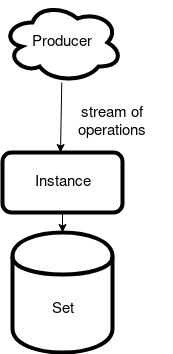
\includegraphics[width=0.2\textheight]{benchmark-single.png}
\end{figure}
\begin{figure}[ht]
\centering
\caption{Multiple processes handling operations from a producer, using locks to handle the shared data structure}
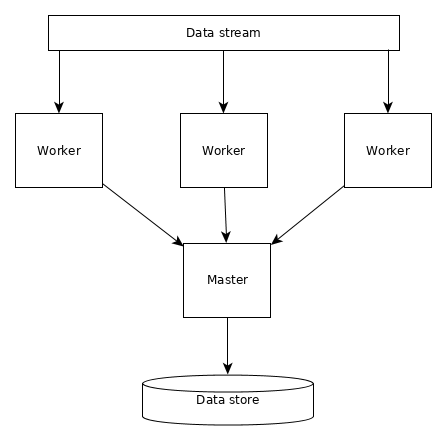
\includegraphics[width=0.3\textheight]{benchmark-serial.png}
\end{figure}
\begin{figure}[ht]
\centering
\caption{Multiple processes handling operations from a producer, using mergeaable types storage to handle the shared data structure}
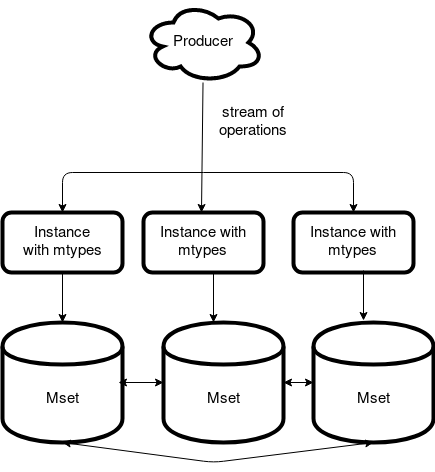
\includegraphics[width=0.3\textheight]{benchmark-mtyped.png}
\end{figure}

\newpage
\bibliographystyle{acm}
\bibliography{all}

\end{document}